\begin{figure}
     \centering
     \begin{subfigure}{0.45\textwidth}
         \centering
         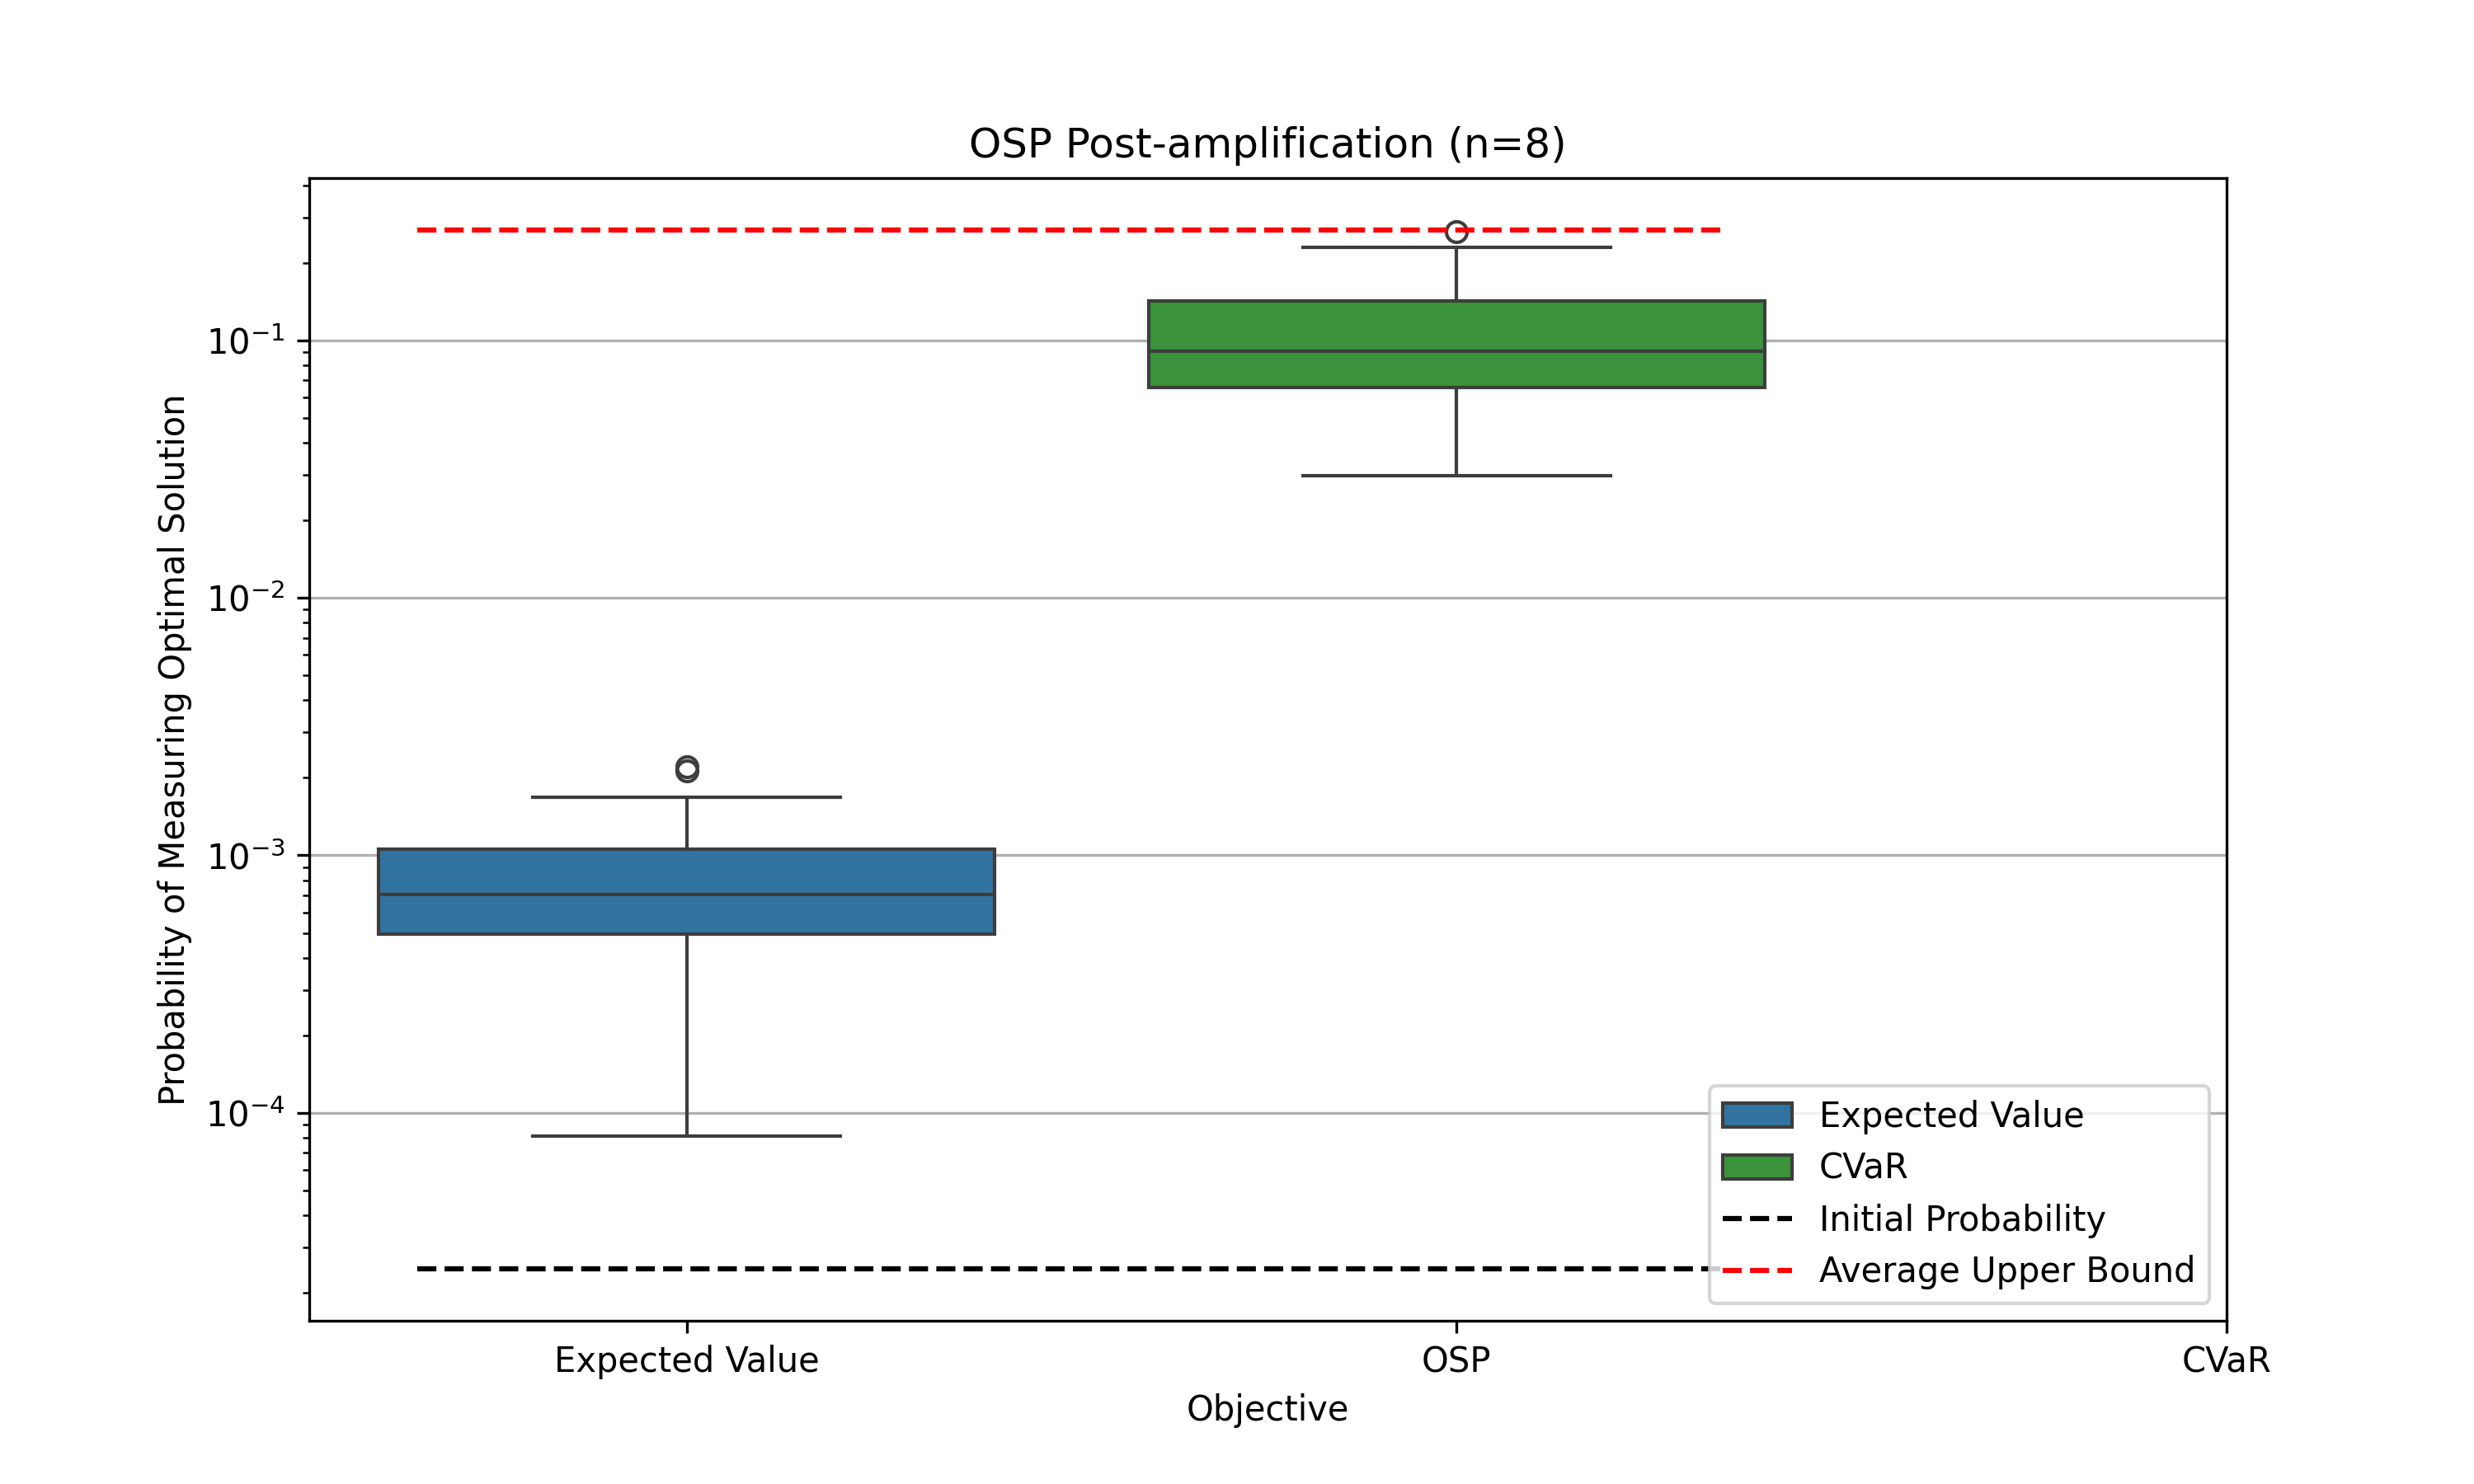
\includegraphics[width=\textwidth]{n=8_prob_optimal_box.png}
         \caption{$n=8$}
         \label{fig:osp 8}
     \end{subfigure}
     \hfill
     \begin{subfigure}{0.45\textwidth}
         \centering
         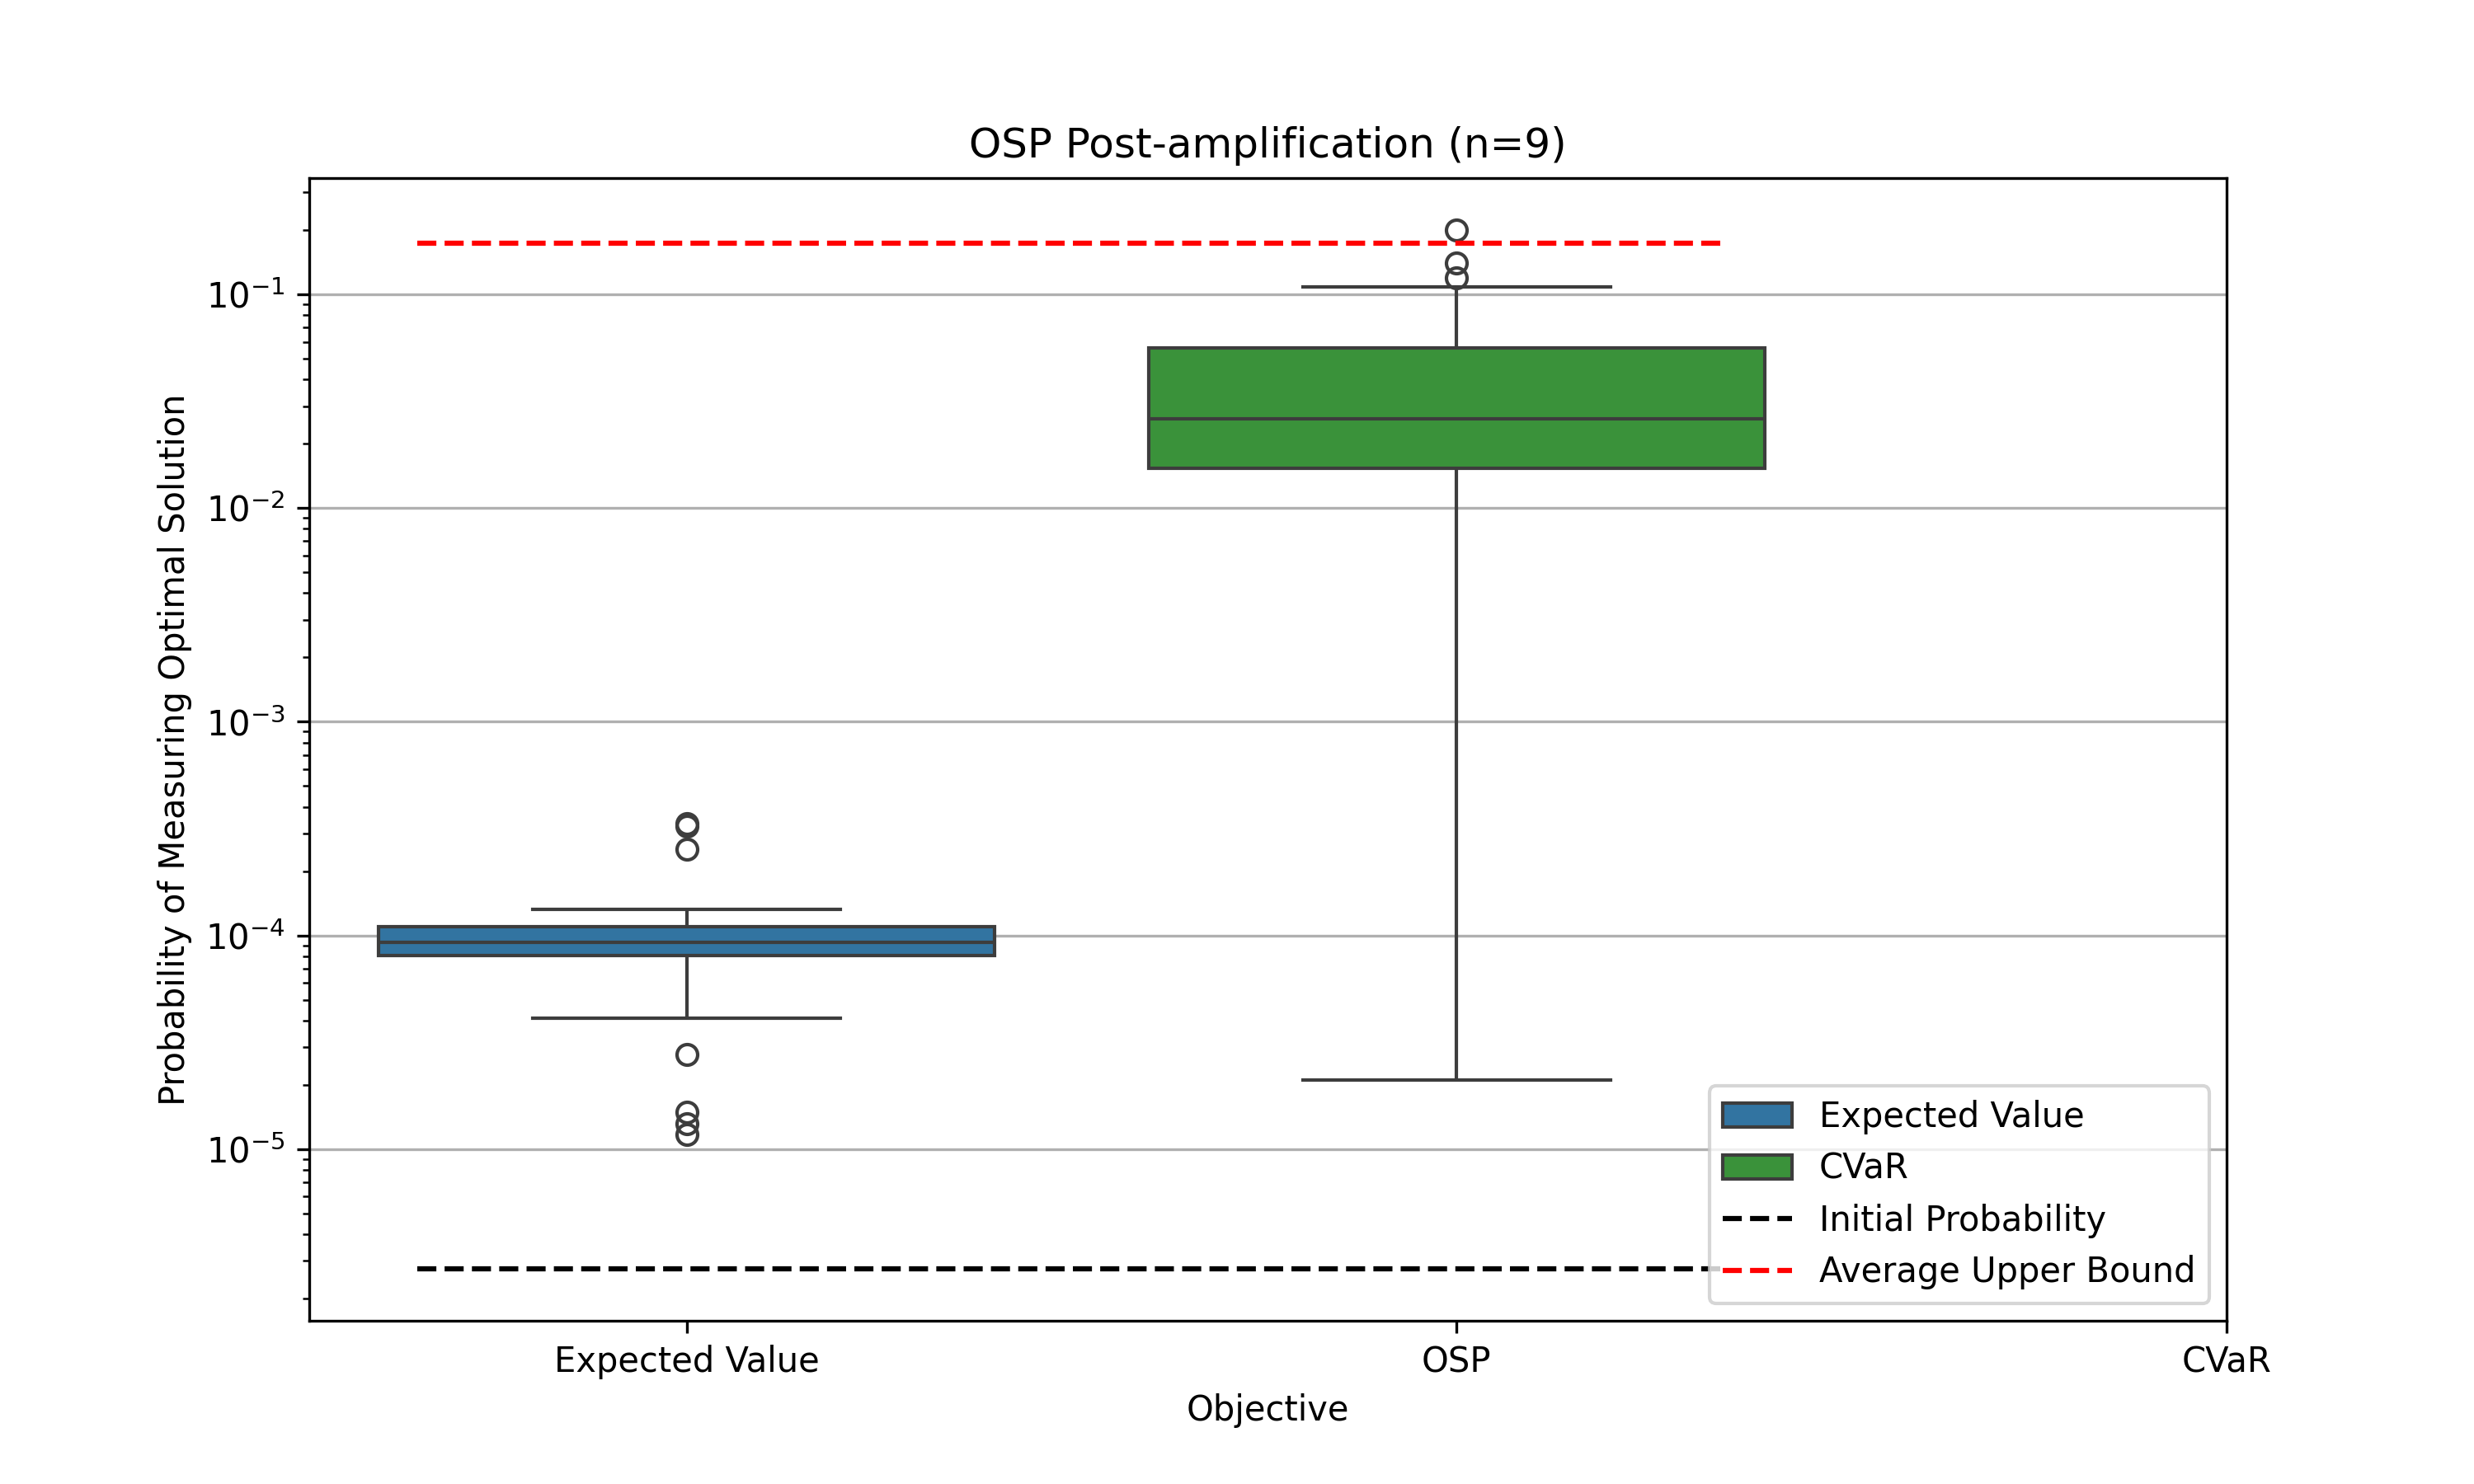
\includegraphics[width=\textwidth]{n=9_prob_optimal_box.png}
         \caption{$n=9$}
         \label{fig:osp 9}
     \end{subfigure}
     \hfill
     \begin{subfigure}{\textwidth}
         \centering
         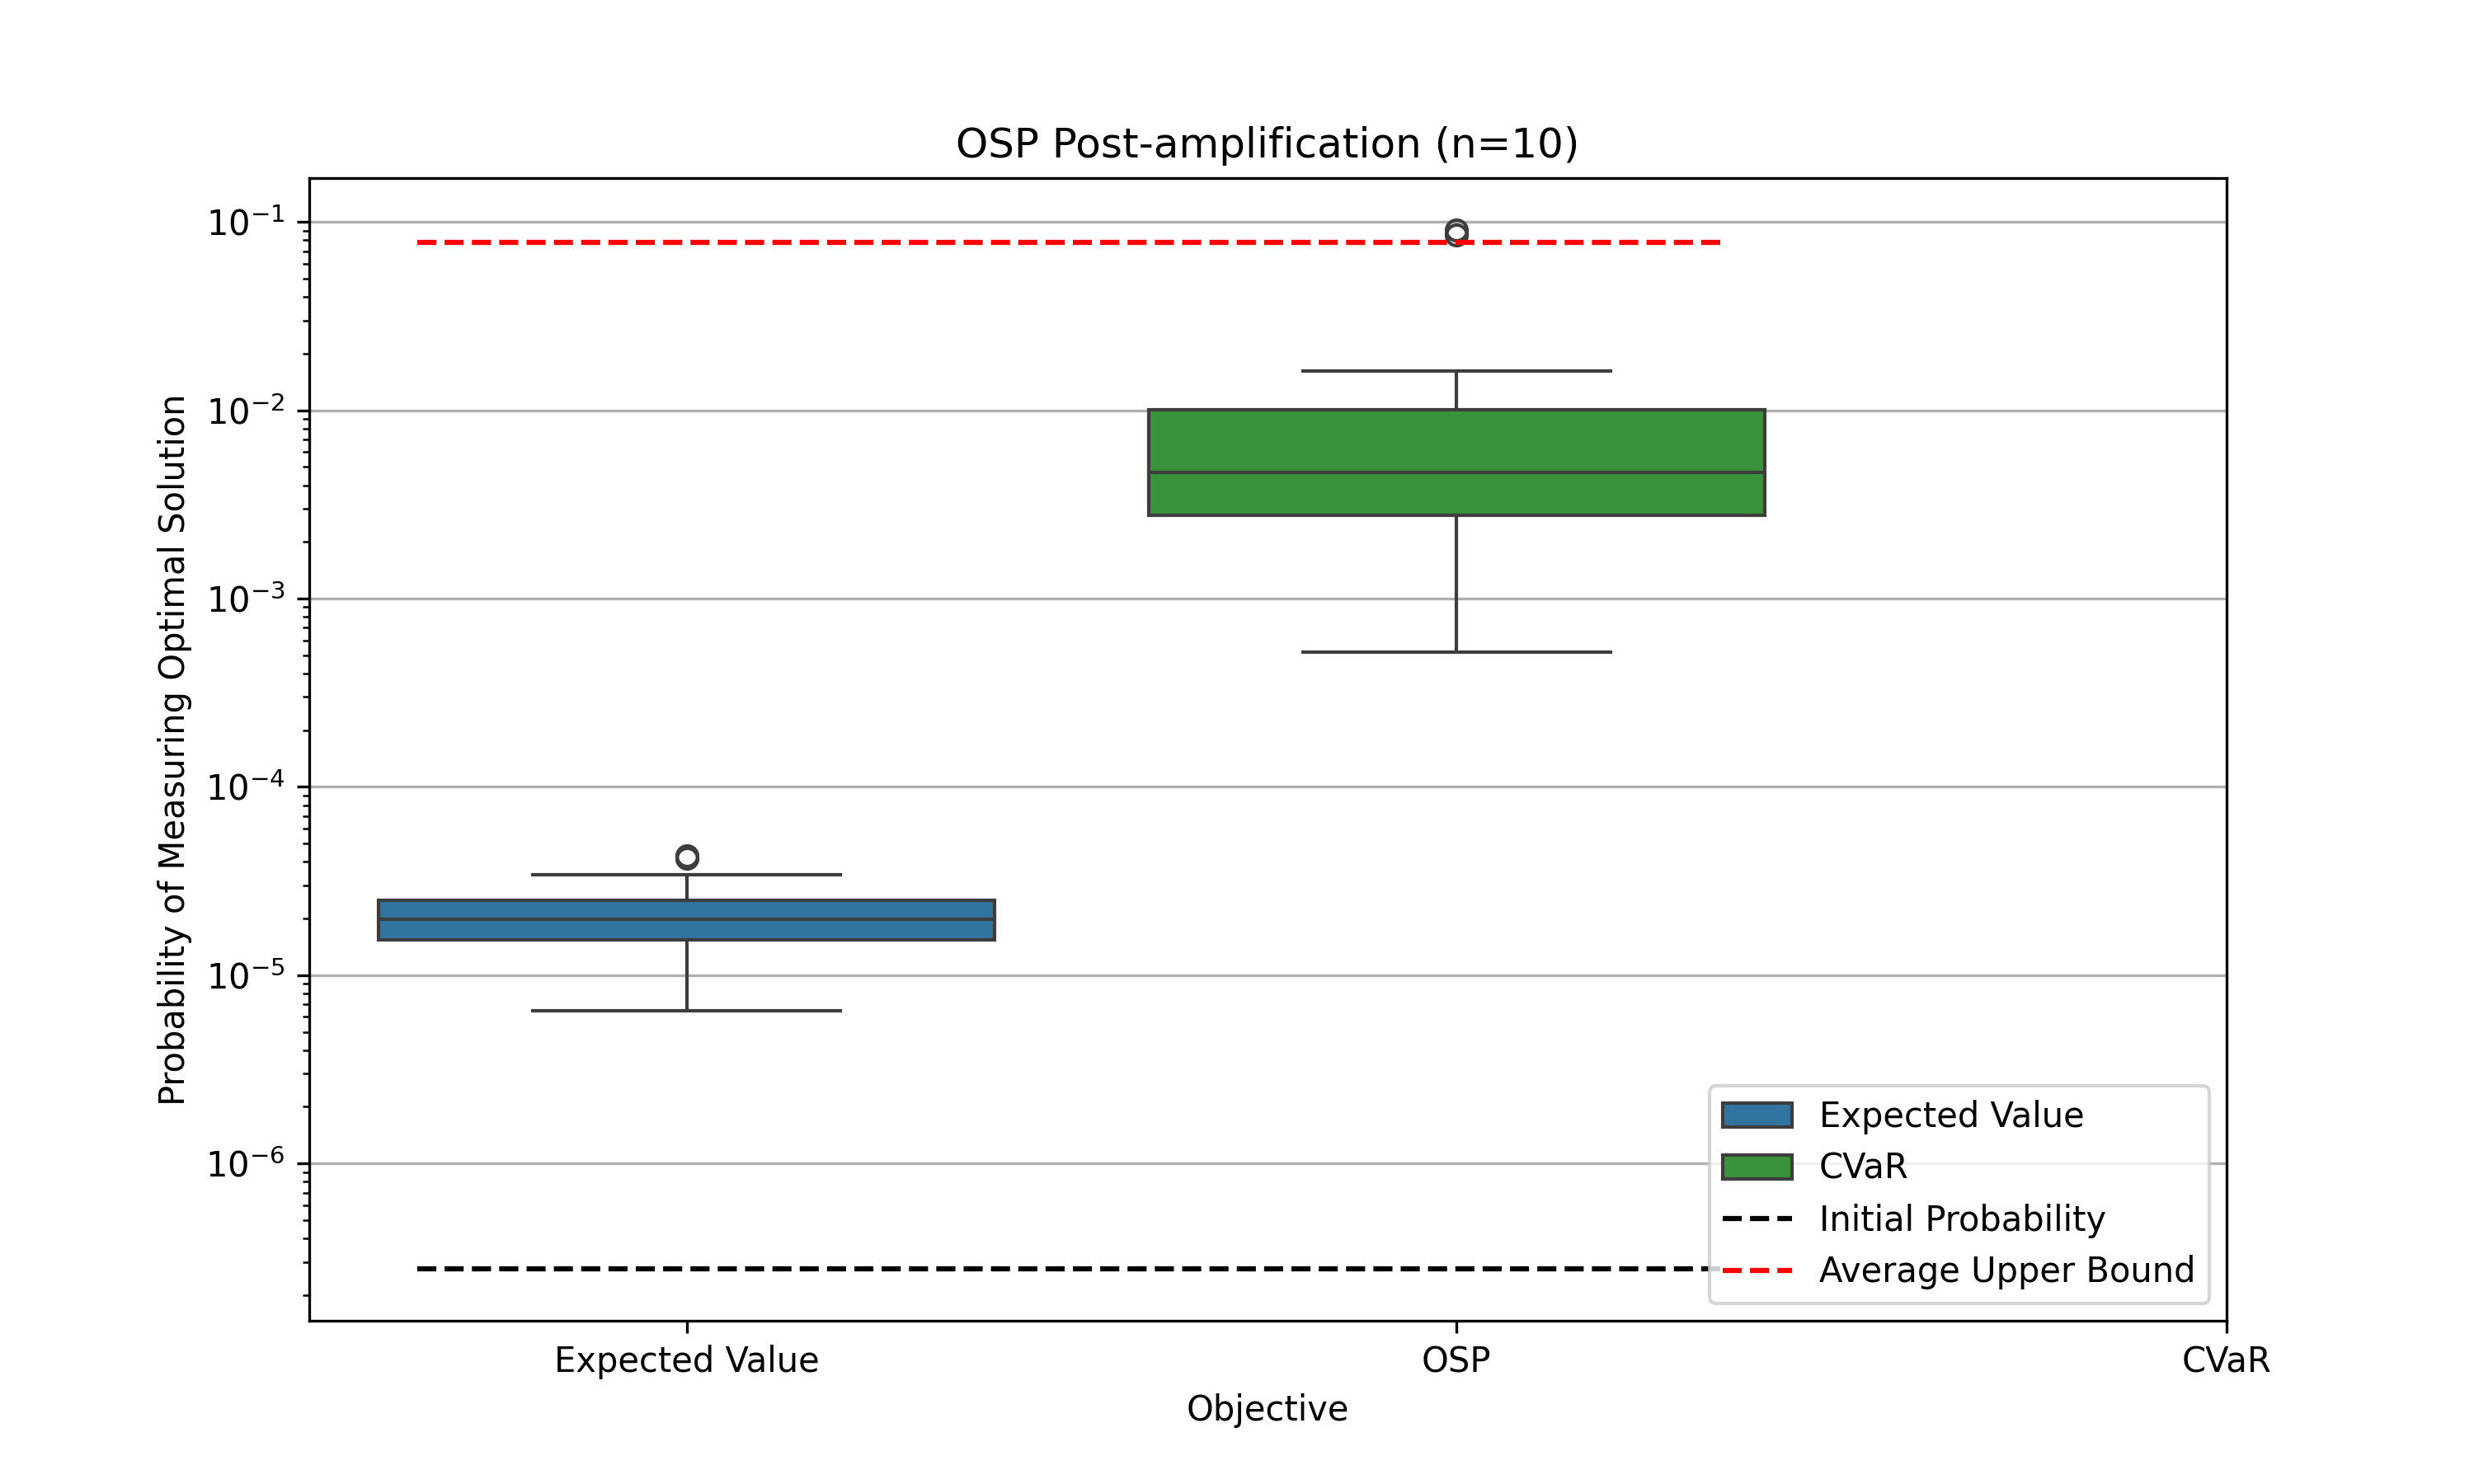
\includegraphics[width=\textwidth]{n=10_prob_optimal_box.png}
         \caption{$n=10$}
         \label{fig:osp 10}
     \end{subfigure}
        \caption{Optimal solution probability (OSP) distributions}
        \label{fig:osp}
\end{figure}


\begin{figure}
     \centering
     \begin{subfigure}{0.45\textwidth}
         \centering
         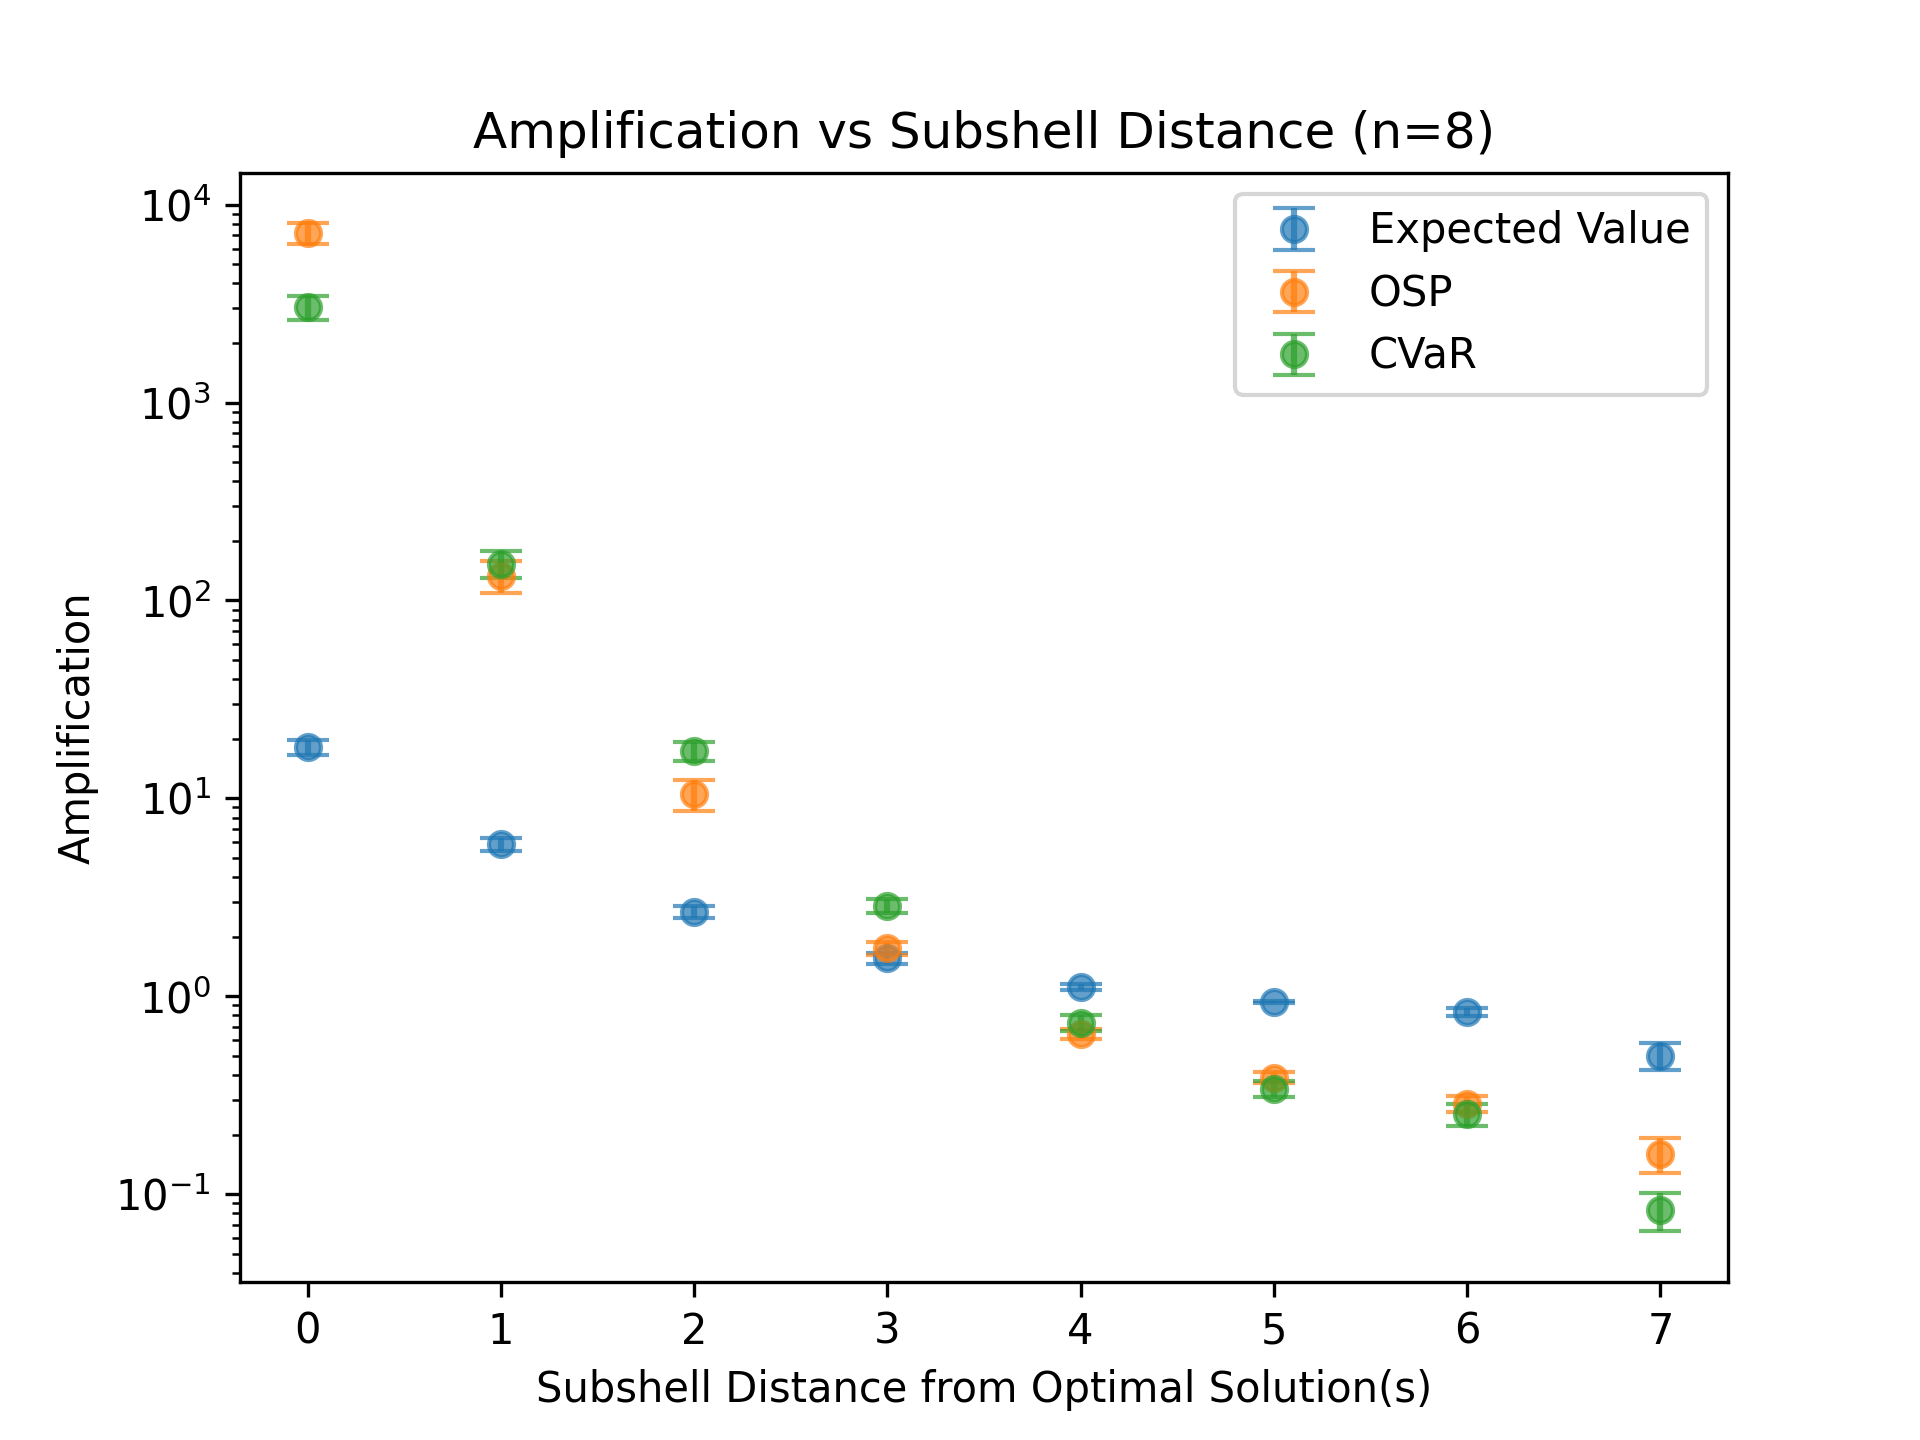
\includegraphics[width=\textwidth]{n=8_amplification_vs_subshell_distance.png}
         \caption{$n=8$}
         \label{fig:amp vs sub 8}
     \end{subfigure}
     \hfill
     \begin{subfigure}{0.45\textwidth}
         \centering
         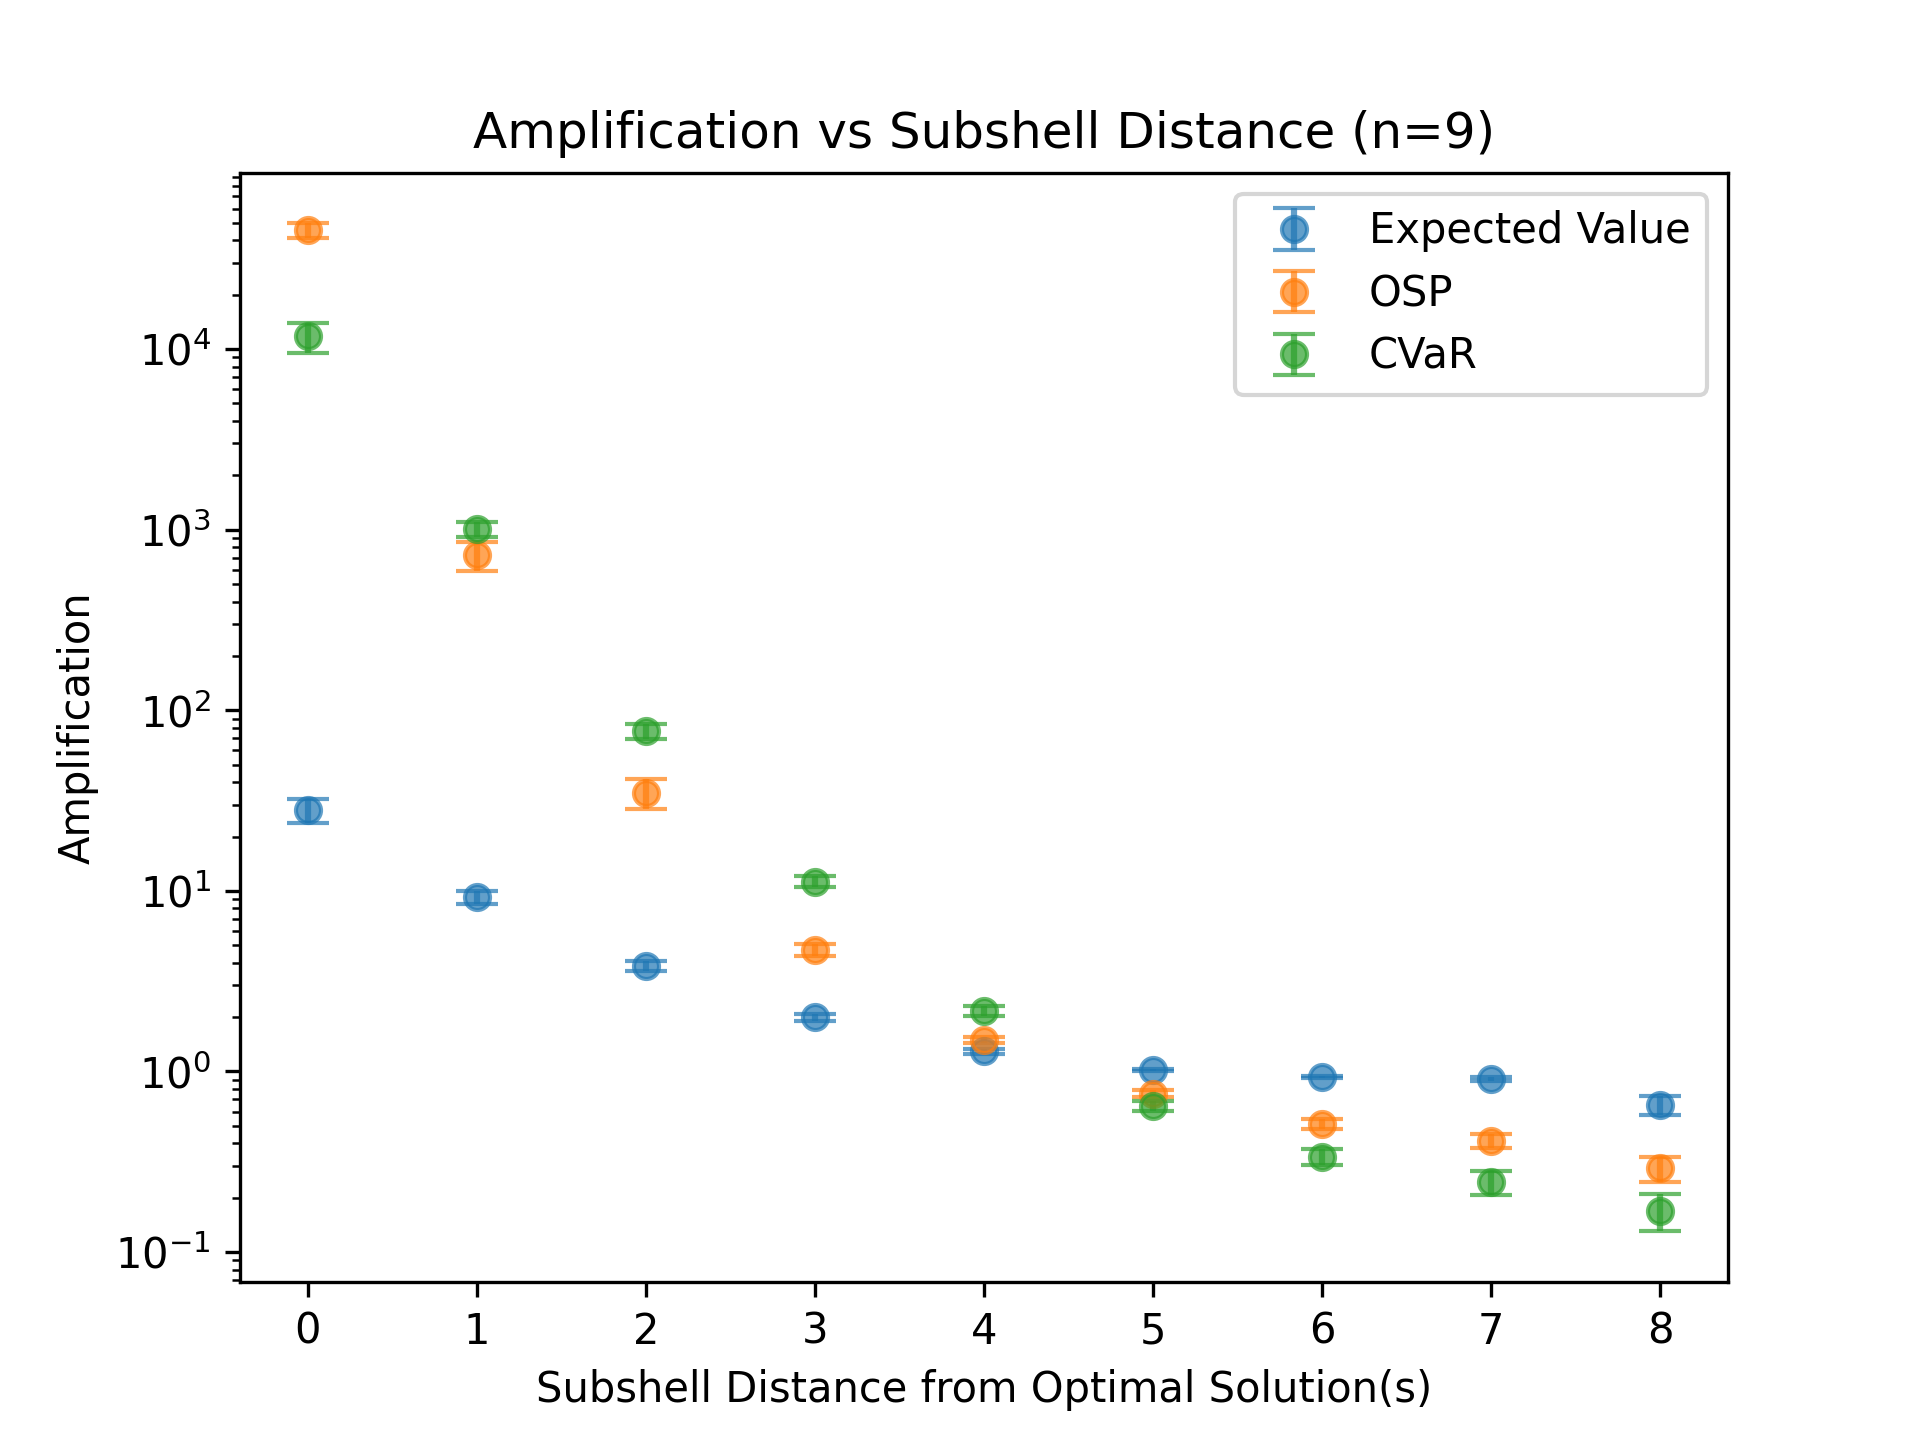
\includegraphics[width=\textwidth]{n=9_amplification_vs_subshell_distance.png}
         \caption{$n=9$}
         \label{fig:amp vs sub 9}
     \end{subfigure}
     \hfill
     \begin{subfigure}{\textwidth}
         \centering
         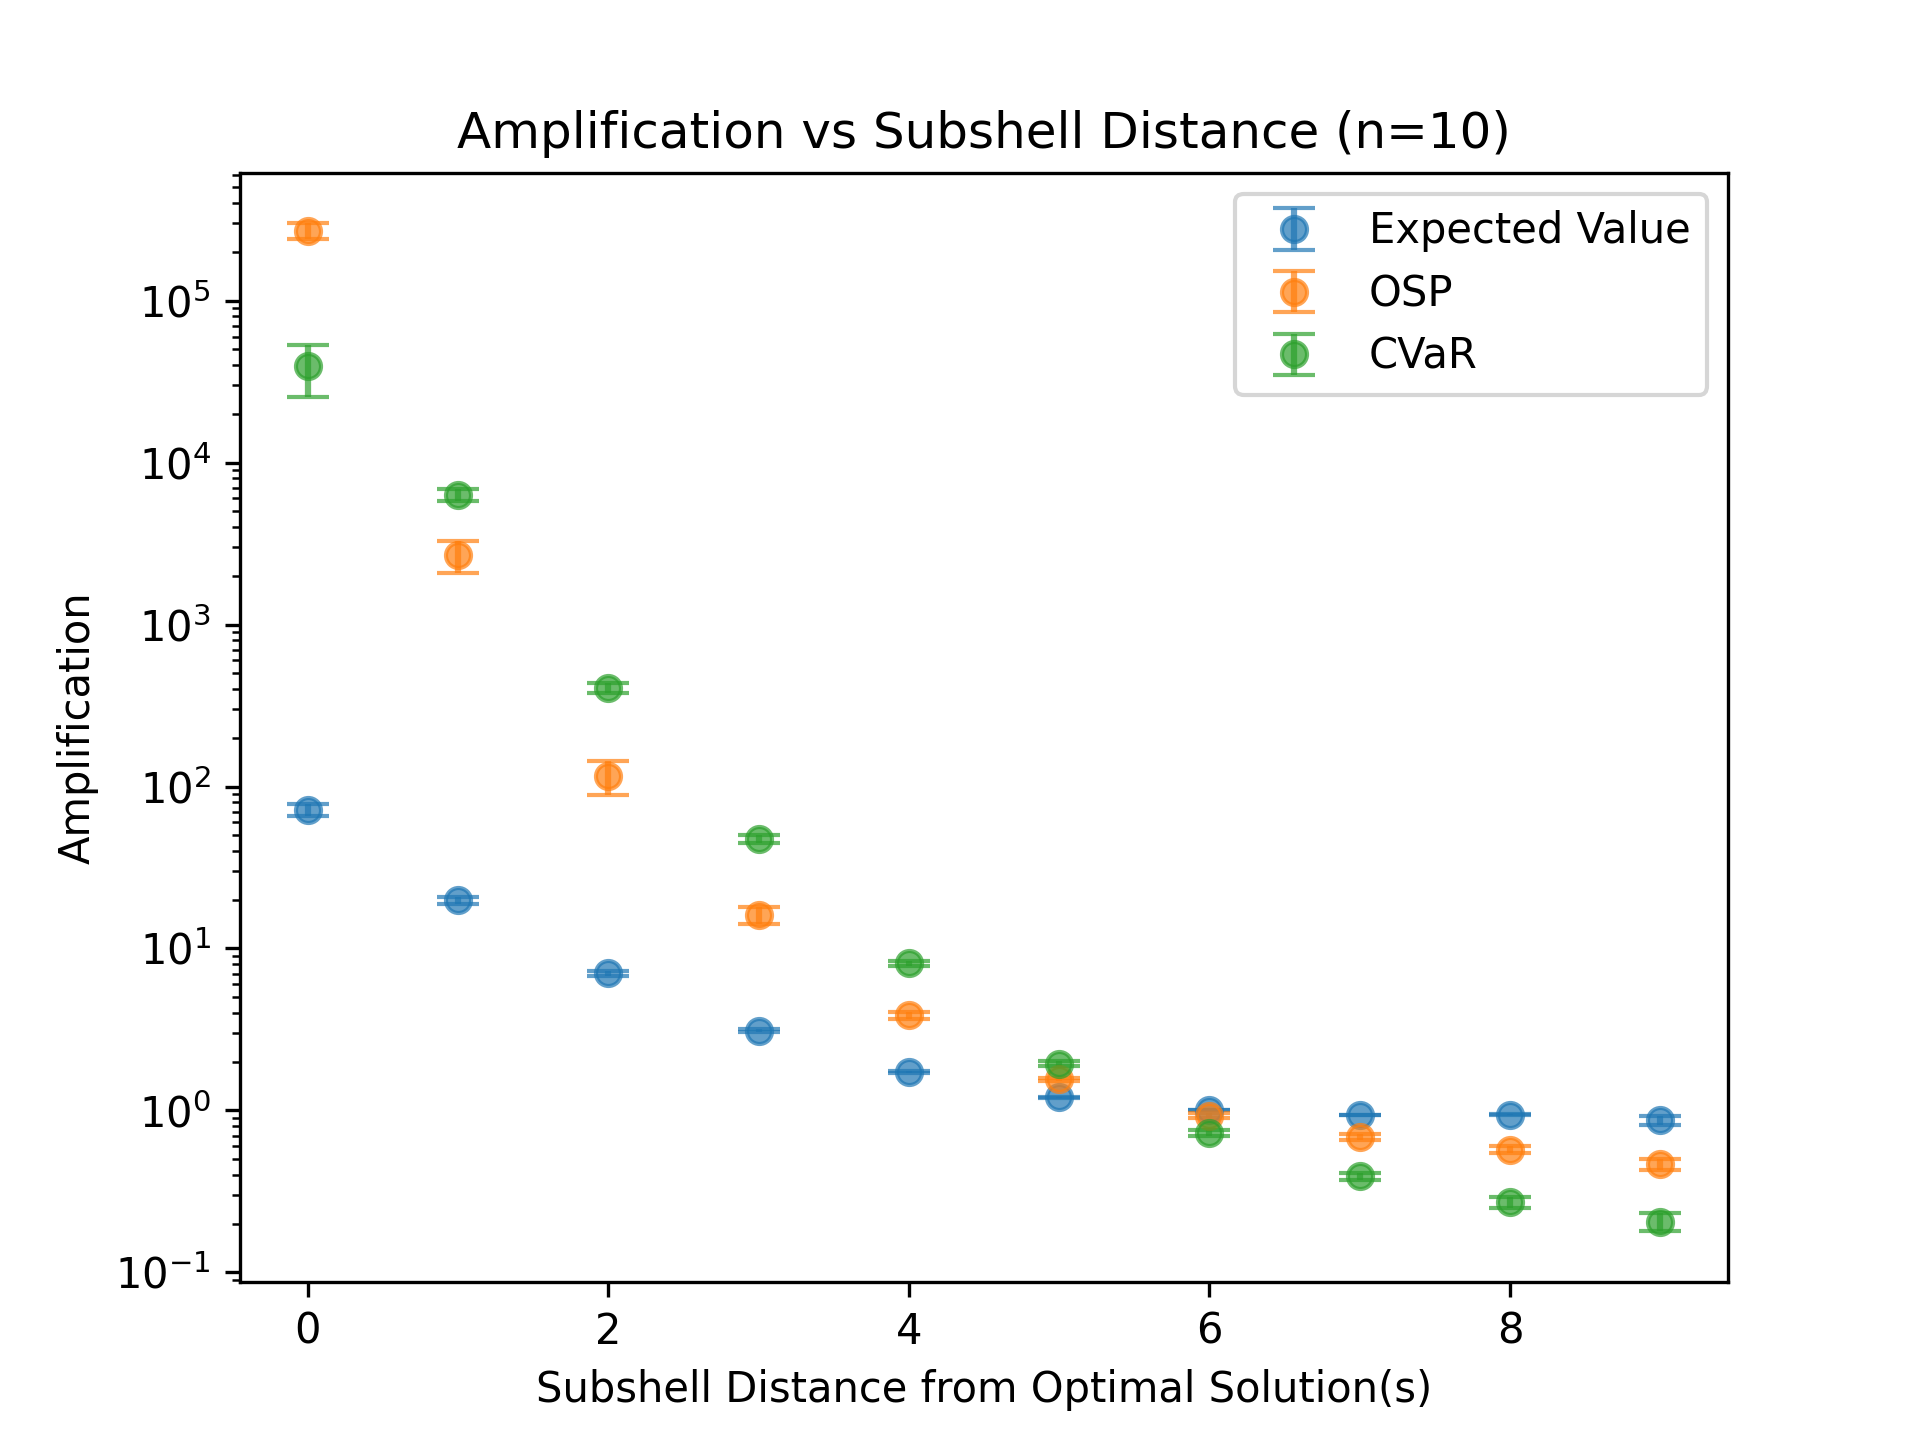
\includegraphics[width=\textwidth]{n=10_amplification_vs_subshell_distance.png}
         \caption{$n=10$}
         \label{fig:amp vs sub 10}
     \end{subfigure}
        \caption{Mean amplification applied to each solution grouped by their distance from the optimal solution.}
        \label{fig:amp vs sub}
\end{figure}